

\chapter{Appendix A}
\label{app:A}

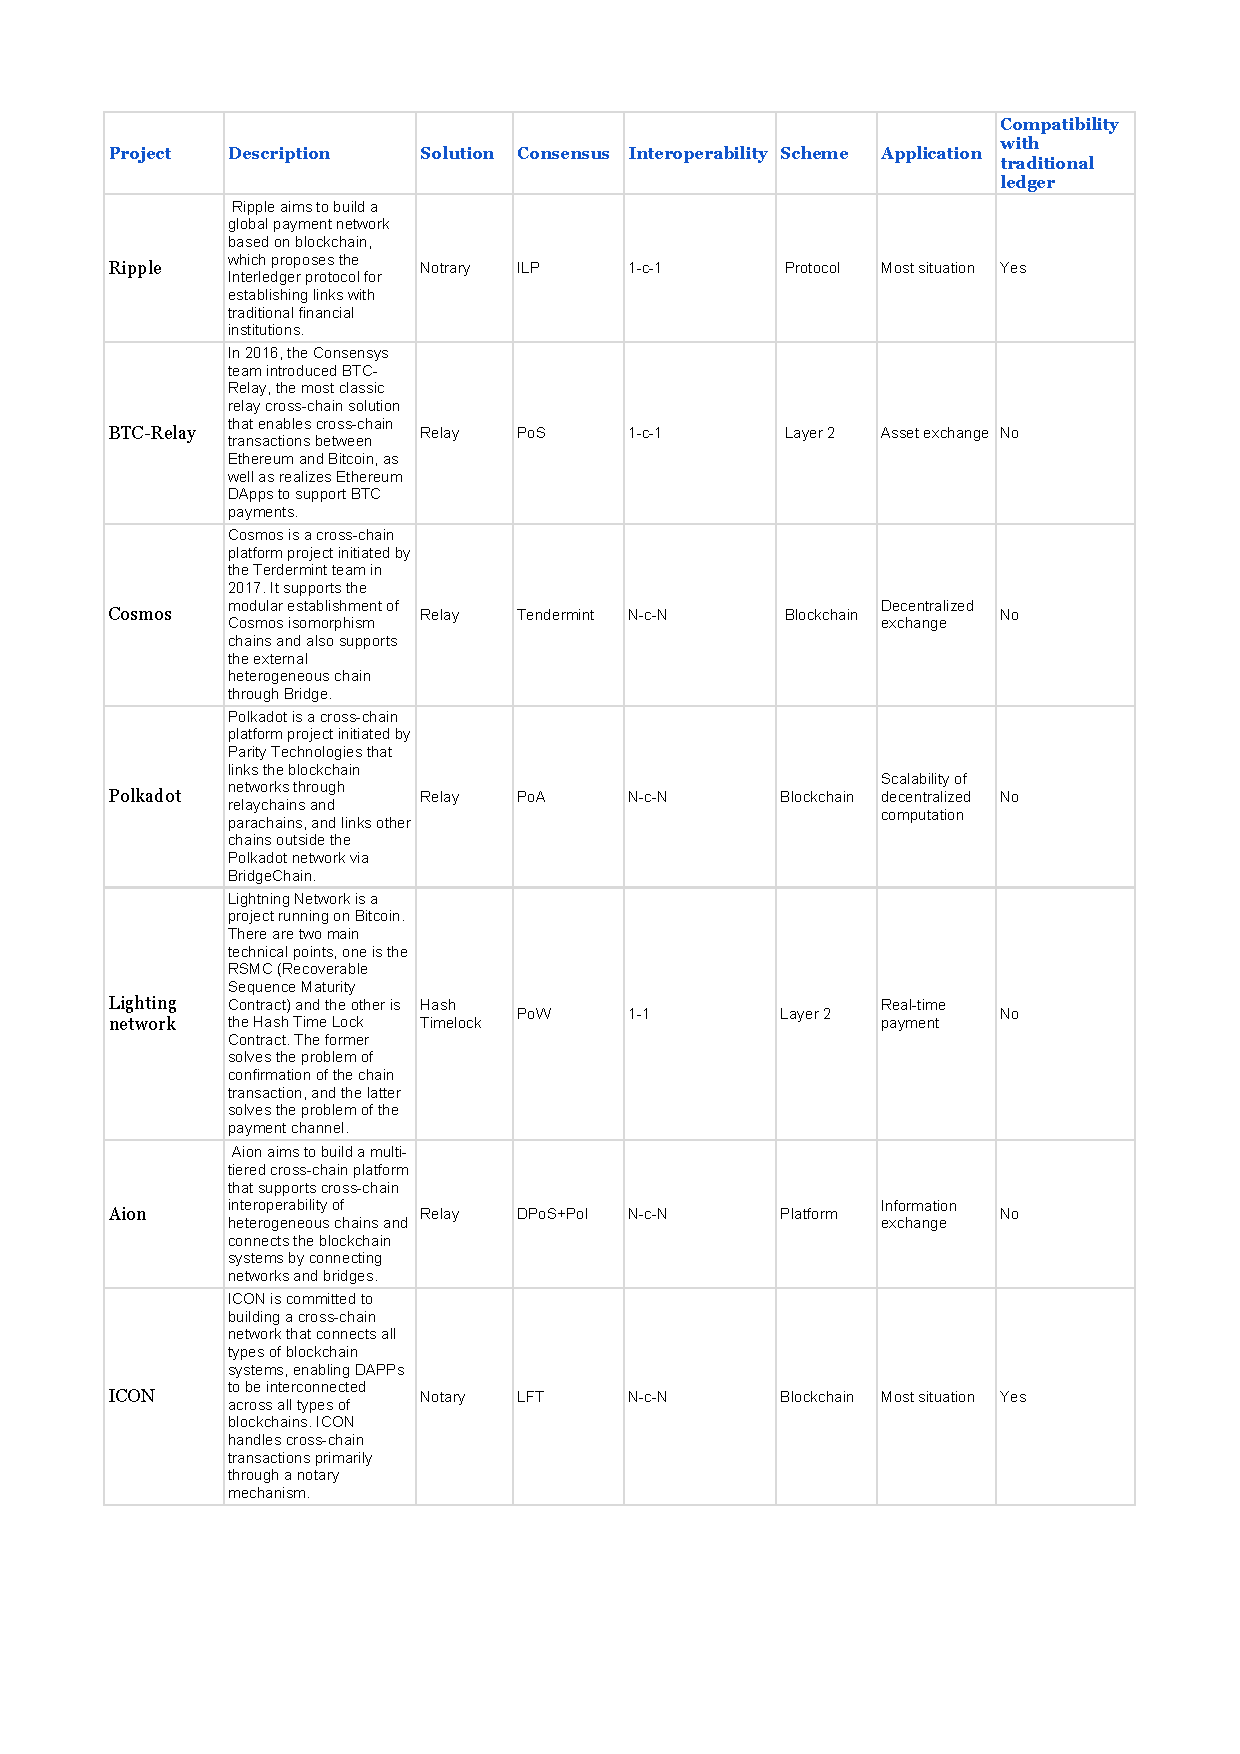
\includepdf[pages={1,2,3}]{table.pdf} 
\captionof{table}{A comparison table of 20 cross-chain projects} 

\noindent In the table above, the level of interoperability\footnotemark[1] is defined by using the following notation:
\begin{itemize}
    \item 1-c-1: Two connected blockchains per time with a connector;
    \item N-c-N: Many connected blockchains per time with connectors;
    \item 1-1: Two connected blockchain connected per time without connector;
    \item N-N: Many connected blockchains per time without connectors.
\end{itemize}




     \footnotetext[1]{This concept is adopted from Quant Overledger White paper\cite{verdian2018quant}}
    %\footnotetext[1]{HHCM: Hierarchical Hybrid Consensus Mechanism}



